\subsection{\textit{Front-end}}
\subsubsection{\textit{Root} della \textit{repository} e \textit{file} di configurazione}

\begin{figure}[H]
      \centering
      %\hspace{-3.25cm} % Sposta la figura a sinistra di n cm
      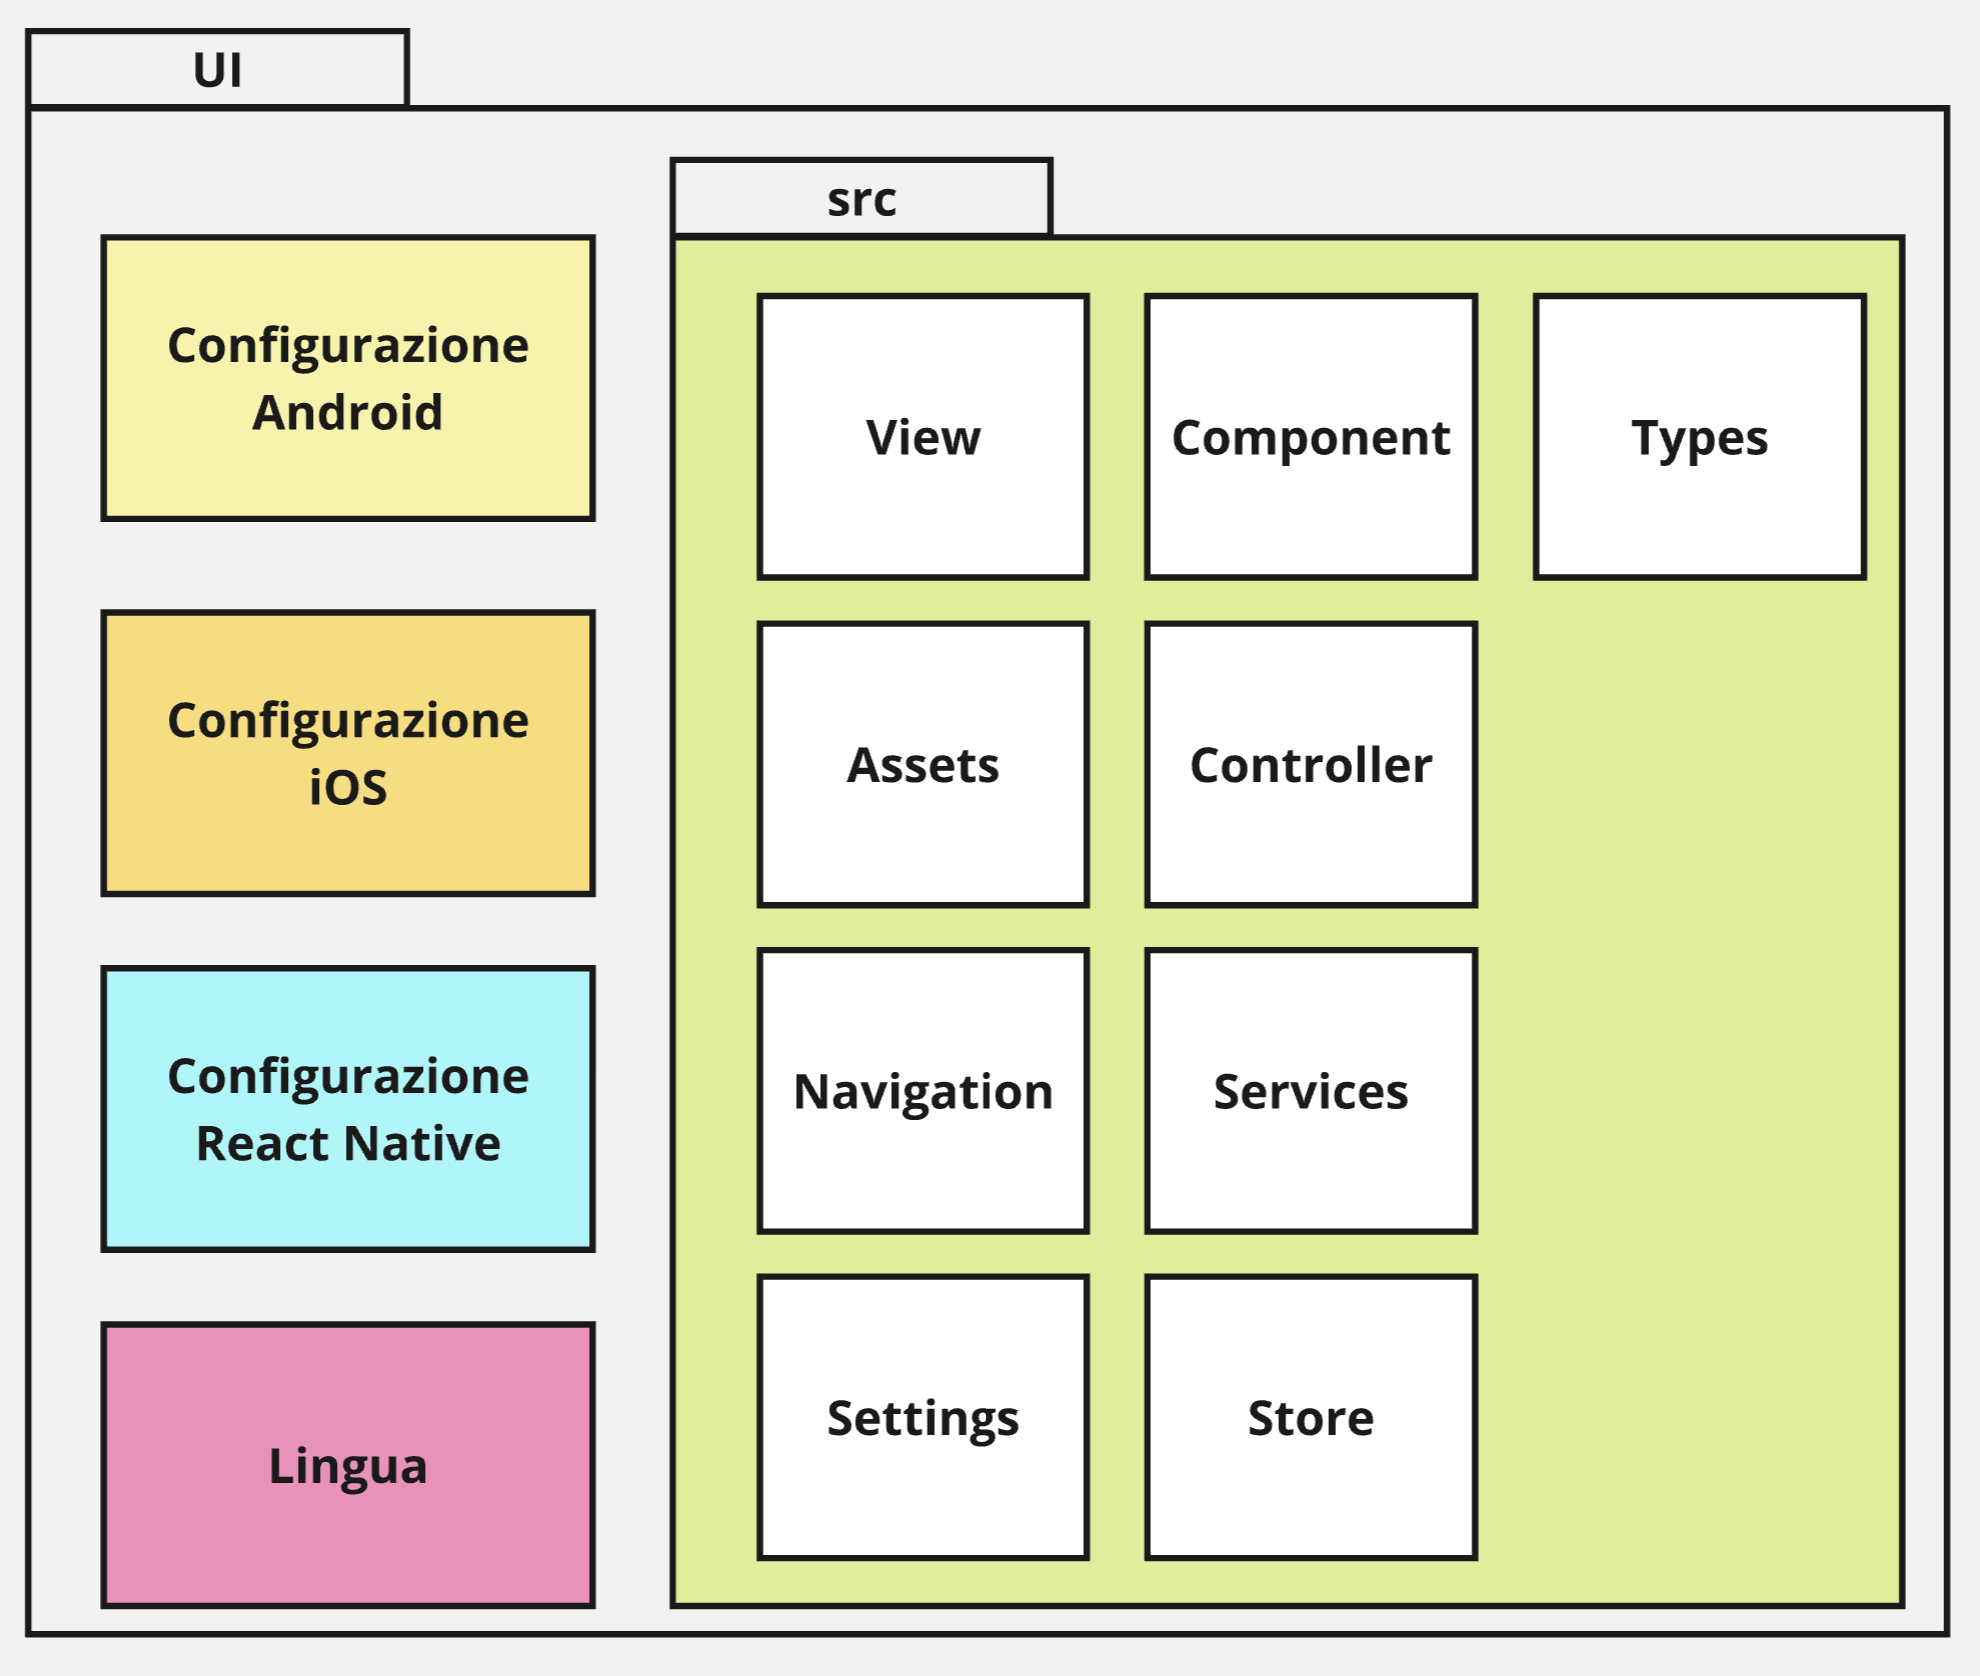
\includegraphics[width=0.6\textwidth]{img/architettura_ui.png}
      \caption{\textit{Root} della \textit{repository} che contiene il \textit{front-end}}
      \label{fig:ui architecture}
\end{figure}

Infine ho studiato React Native e l'architettura utilizzata per il \textit{front-end}.\\
Prima di descrivere l'architettura soffermiamoci ad analizzare il contenuto del \textit{root} della \textit{repository} 
mostrata dalla figura \ref{fig:ui architecture}.
Qui sono contenuti i file di configurazione di React Native e le impostazioni dei compilatori.\\
La \textit{repository} è suddivisa nelle seguenti cartelle:
\begin{itemize}
    \item \texttt{\textbf{Android}}: specifica per React Native, contiene i file di configurazione 
          per la versione Android dell'\textit{app} e \textit{file} come \texttt{build.gradle} e \texttt{AndroidManifest.xml} 
          per la configurazione del compilatore Android;
    \item \texttt{\textbf{iOS}}: specifica per React Native, contiene il progetto Xcode e i file di configurazione 
          per la versione iOS dell'\textit{app} e \textit{file} per la configurazione del compilatore di iOS;
    \item \texttt{\textbf{lang}}: contiene i \textit{file} \texttt{en.json e it.json} che definiscono il testo usato nell'
          applicazione nelle lingue italiano e inglese;
    \item \texttt{\textbf{src}}: contiene tutto il codice del \textit{front-end} e realizza l'architettura modulare;
    \item \textbf{Altri \textit{file} di configurazione}: questi \textit{file} sono fondamentali 
          per garantire un corretto funzionamento e una gestione efficiente del progetto, qui riporto quelli più importanti:
          \begin{itemize}
            \item \textbf{\texttt{package.json}}: contiene le informazioni sul progetto come il nome del progetto, versione,
                  \textit{script} di comando e dipendenze. È il \textit{file} principale per gestire i pacchetti Node.js utilizzati nel progetto;
            \item \textbf{\texttt{yarn.lock}}: questo \textit{file} viene generato automaticamente quando si genera il progetto e 
                  permette di gestire ed installare le dipendenze con le loro versioni esatte;
            \item \textbf{\texttt{metro.config.js}}: configura Metro, il \textit{bundler} di JavaScript predefinito 
                  per React Native. Un \textit{bundler} è uno strumento di sviluppo \textit{software} che combina diversi 
                  \textit{file} di codice sorgente e le loro dipendenze in uno o più \textit{file} ottimizzati, pronti per essere distribuiti 
                  o eseguiti in un ambiente di produzione. Questo \textit{file} permette di personalizzare il comportamento di Metro, come 
                  l'aggiunta di alias, path customizzati, o l'esclusione di determinati \textit{file} dalla \textit{build}.
            \item \textbf{\texttt{babel.config.js}}: configura Babel, il \textit{transpiler} di JavaScript. 
                  Definisce come il codice deve essere trasformato per essere compatibile con le varie versioni di JavaScript e i 
                  diversi ambienti in cui verrà eseguito.
            \item \textbf{\texttt{index.js}}: punto d'ingresso principale dell'applicazione React Native. Qui viene 
                  avviato il \textit{rendering} del componente radice dell'\textit{app};
            \item \textbf{\texttt{app.tsx}}: contiene il componente radice dell'applicazione. Qui vengono definiti l'interfaccia 
                  utente principale e la logica di base dell'\textit{app}.
            \item \textbf{\texttt{tsconfig.json}}: configura il compilatore TypeScript, specificando le opzioni di compilazione 
            e il comportamento del \textit{transpiling} del codice TypeScript in JavaScript.
          \end{itemize}
\end{itemize}
\subsubsection{Architettura modulare}

\begin{figure}[H]
      \centering
      %\hspace{-3.25cm} % Sposta la figura a sinistra di n cm
      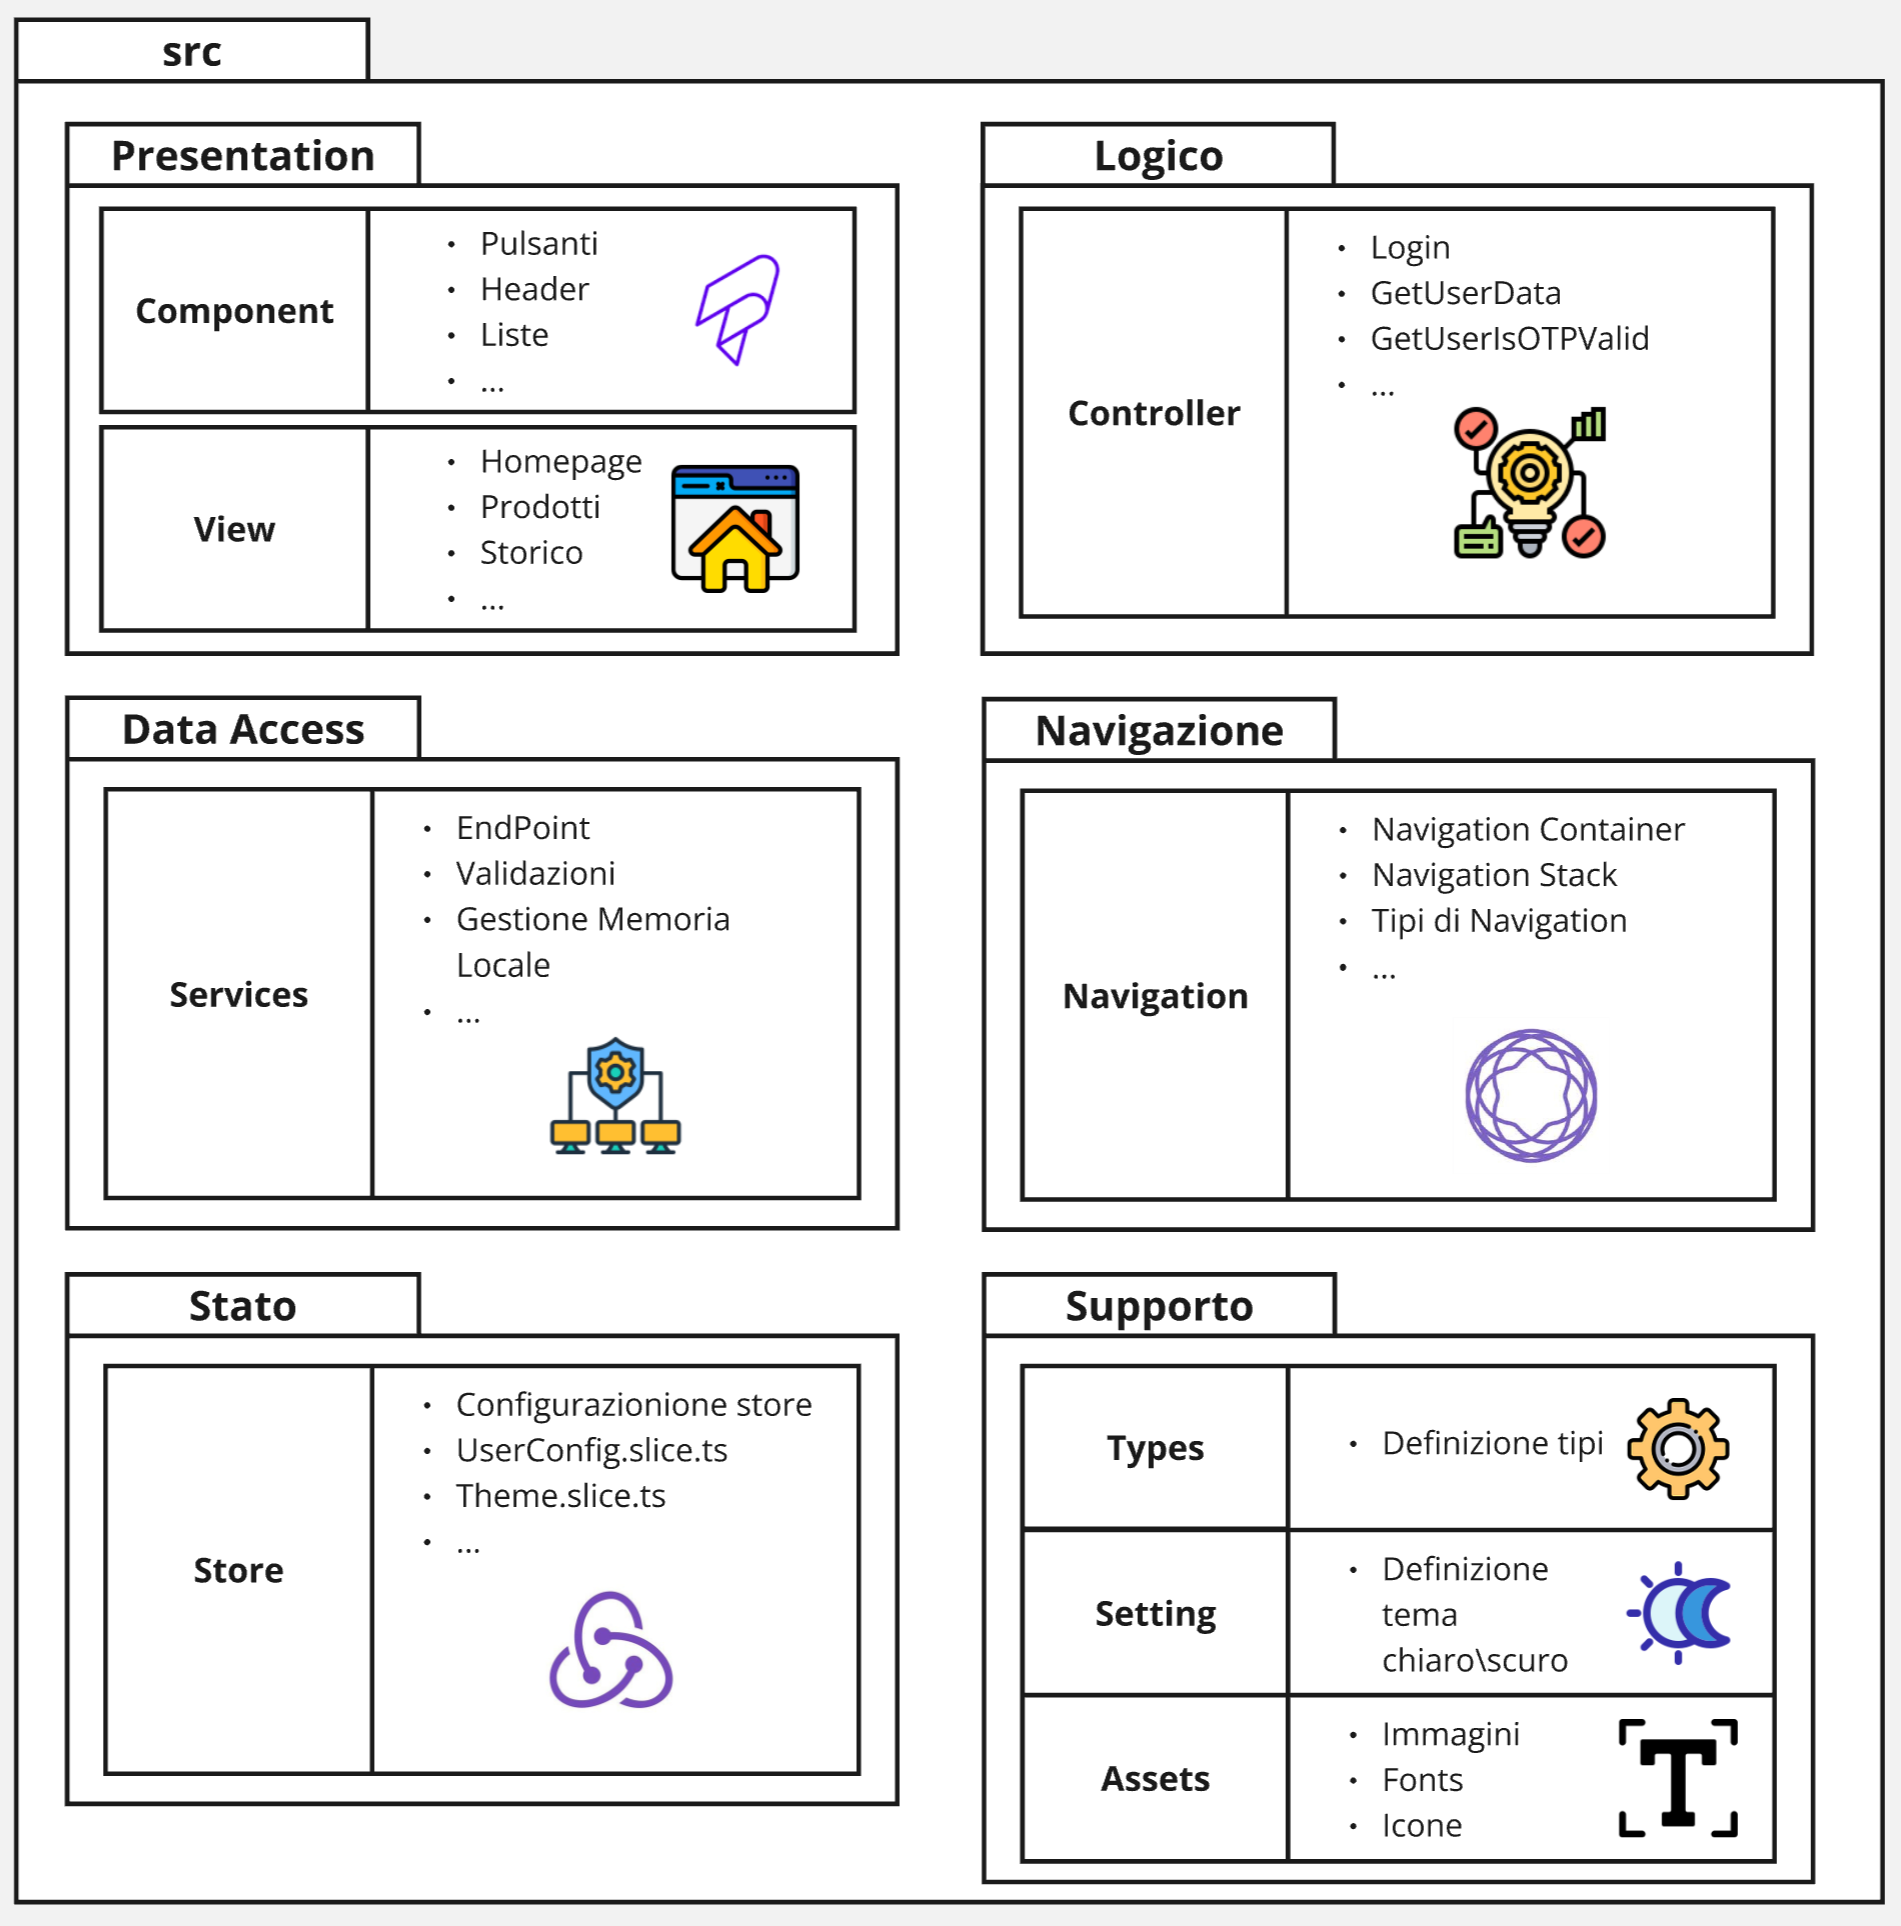
\includegraphics[width=0.8\textwidth]{img/modules_architecture.png}
      \caption{Rappresentazione dell'architettura modulare per {\movi}}
      \label{fig:frontend architecture}
\end{figure}

L'applicazione implementa un'architettura modulare, un approccio di progettazione \textit{software} che, come mostra 
la figura \ref{fig:frontend architecture}, separa le 
funzionalità in moduli indipendenti e intercambiabili. Questa architettura è particolarmente adatta alle applicazioni 
React Native, consentendo una maggiore flessibilità, manutenibilità e scalabilità del codice.
I moduli sono:
\begin{itemize}
      \item \textbf{Moduli di \textit{presentation}}: le componenti grafiche che realizzano l'interfaccia dell'\textit{app}. 
            Per favorire la riusabilità del codice sono divise in due cartelle \texttt{View} e \texttt{Component}. In 
            \texttt{Component} vengono definiti i componenti e il loro stile, che vengono usati per comporre le viste 
            definiti in \texttt{View} che contengono anche la logica dei componenti che la compongono;
      \item \textbf{Modulo logico}: contiene la logica di \textit{business} dell'applicazione, è contenuto nella 
            cartella \texttt{Controller};
      \item \textbf{Modulo di accesso ai dati}: contiene la definizione degli \textit{endpoint} che permettono la 
            connessione alle \gls{api} e la gestione della memoria locale del dispositivo, è contenuto nella cartella 
            \texttt{Services};
      \item \textbf{Modulo di gestione dello stato}: centralizza la gestione dello stato utilizzando 
            la libreria React Native Redux, è contenuto nella cartella \texttt{Store};
      \item \textbf{Modulo di navigazione}: gestisce il \textit{routing} e la navigazione tra le diverse 
            schermate dell'\textit{app}, implementato tramite la libreria React Native Navigation è 
            contenuto nella cartella \texttt{Navigation};
      \item \textbf{Moduli di supporto}: diviso in tre \textit{directory}: \texttt{Types} dove sono 
            definiti i tipi usati all'interno dell'applicazione, \texttt{Assets} dove sono raccolte 
            le risorse statiche (come le immagini, le icone, ecc.) e \texttt{Settings} dove sono definiti 
            i temi chiaro e scuro dell'\textit{app}.
\end{itemize}
Questo approccio si adatta bene alla natura \textit{component-based} di React Native, permettendo una chiara 
separazione delle responsabilità e una struttura del codice organizzata e intuitiva.